\section{机械运动的分类}\label{sec:3-2}

\begin{wrapfigure}[11]{r}{5cm}
    \centering
    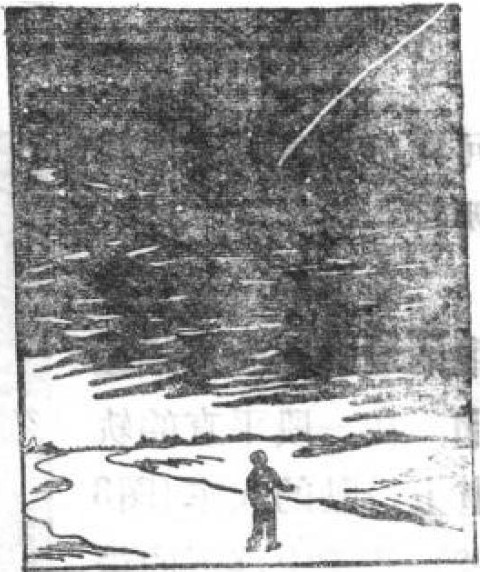
\includegraphics[width=4cm]{../pic/czwl1-ch3-1}
    \caption{}\label{fig:3-1}
\end{wrapfigure}

我们平常看到的机械运动是各种各样的,有的物体沿直线运动,有的物体沿曲线运动,
有的物体运动得很快,有的物体运动得很慢,有的物体在运动中时快时慢。
为了进一步研究机械运动,需要先对机械运动进行分类。

物体从一个位置运动到另一个位置,总是要经过一定的路线。有时物体经过的路线是可以看见的,
例如秋夜看到的流星的长长的印迹,就是它经过的路线(图 \ref{fig:3-1})。
航空表演时高空中的飞机拉出的白烟,就是飞机飞过的路线。
运动路线虽然有多种多样,但总是可以分为直线和曲线两种。

经过的路线是直线的运动叫做\textbf{直线运动}。
在一段平直的轨道上行驶的火车(图 \ref{fig:3-2}),从手中落下的粉笔,做的都是直线运动。
经过的路线是曲线的运动叫做\textbf{曲线运动}。
在弯曲跑道上赛车的运动员( 图 \ref{fig:3-3}),在转弯处行驶的汽车,做的都是曲线运动。
直线运动比较简单,我们在下面只研究直线运动。

\begin{figure}[htbp]
    \centering
    \begin{minipage}{8cm}
    \centering
    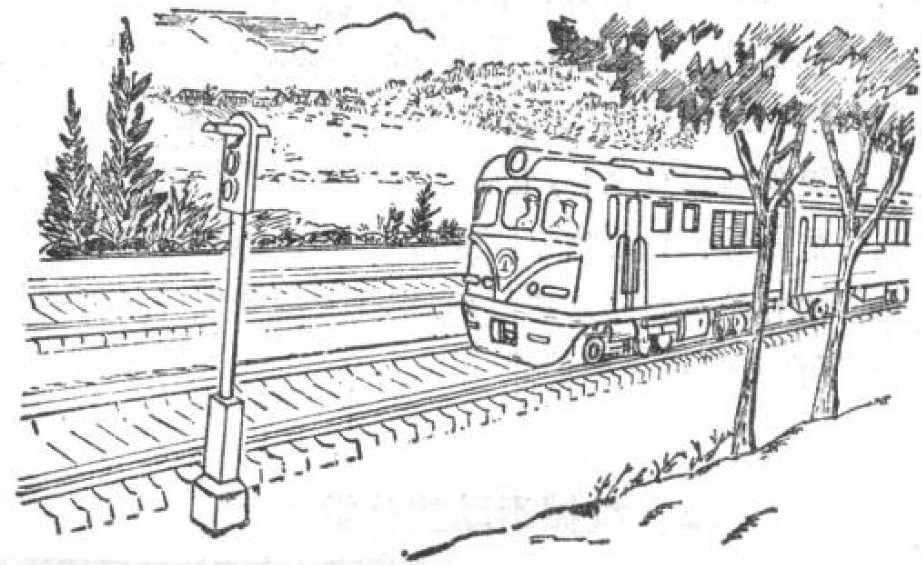
\includegraphics[width=8cm]{../pic/czwl1-ch3-2}
    \caption{}\label{fig:3-2}
    \end{minipage}
    \qquad
    \begin{minipage}{4cm}
    \centering
    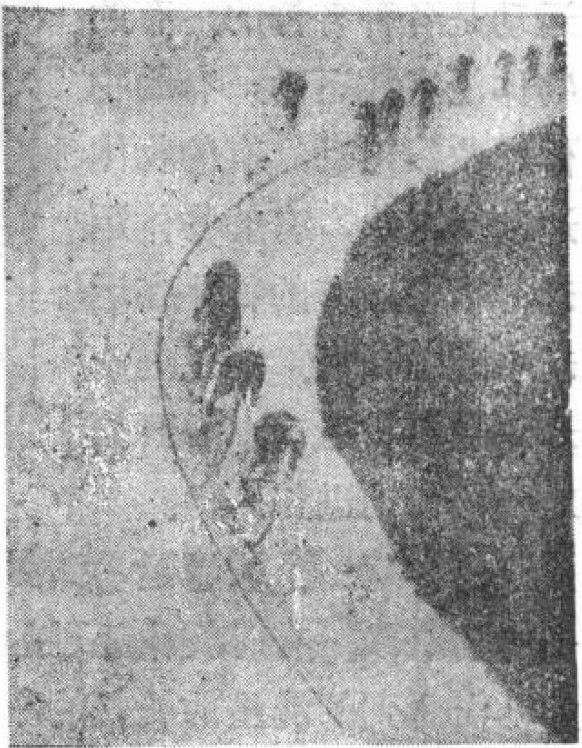
\includegraphics[width=4cm]{../pic/czwl1-ch3-3}
    \caption{}\label{fig:3-3}
    \end{minipage}
\end{figure}


在一段时间内,运动物体经过的路线的长度,叫做它在这段时间内通过的\textbf{路程},
路程用长度的单位来计量。

汽车在一段平直的公路上运动,如果每小时通过的路程都是 60 千米,每半小时通过的路程都是 30 千米,
每 10 分钟通过的路程都是 10 千米,每一分钟通过的路程都是 1 千米,
我们就说汽车在做匀速直线运动。
\textbf{物体在一条直线上运动,如果在相等的时间内通过的路程都相等,这种运动就叫做匀速直线运动}。

匀速直线运动是不多的,我们平常看到的运动大多不是匀速的。
例如,火车从车站开出的时候,即使做直线运动,但在相等的时间内通过的路程并不相等,而是越来越长,它做的就不是匀速直线运动。
\textbf{物体在一条直线上运动,如果在相等的时间内通过的路程并不相等,这种运动就叫做变速直线运动}。

可见,直线运动又可以分为匀速直线运动和变速直线运动两种。

